\documentclass[11pt, a4paper]{article}
\usepackage{pdfpages}
\usepackage{parallel}
\usepackage[T2A]{fontenc}
%\usepackage{ucs}
\usepackage[utf8]{inputenc}
\usepackage[english,russian]{babel}
\usepackage{hyperref}
\usepackage{rotating}
\usepackage[inner=2cm,top=1.8cm,outer=2cm,bottom=2.3cm,nohead]{geometry}
%\usepackage{listings}
\usepackage{graphicx}
\usepackage{wrapfig}
\usepackage{longtable}
\usepackage{indentfirst}
\usepackage{array}
\usepackage{tikzsymbols}
\usepackage{soul}
\usepackage[ruled,vlined]{algorithm2e}
\usepackage{qrcode}
\counterwithout{figure}{section} 

\usepackage{url}
\makeatletter
\g@addto@macro{\UrlBreaks}{\UrlOrds}
\makeatother

\newcolumntype{P}[1]{>{\raggedright\arraybackslash}p{#1}}
\frenchspacing
%\usepackage{fixltx2e} %text sub- and superscripts
\usepackage{icomma} % коскі ў матэматычным рэжыме
%\PreloadUnicodePage{4}

\newcommand{\longpage}{\enlargethispage{\baselineskip}}
\newcommand{\shortpage}{\enlargethispage{-\baselineskip}}

\def\switchlang#1{\expandafter\csname switchlang#1\endcsname}
\def\switchlangbe{
\let\saverefname=\refname%
\def\refname{Літаратура}%
\def\figurename{Іл.}%
}
\def\switchlangru{
\let\saverefname=\refname%
\let\savefigurename=\figurename%
\def\refname{Литература}%
\def\figurename{Рис.}%
}
\def\switchlangen{
\let\saverefname=\refname%
\def\refname{References}%
\def\figurename{Fig.}%
}

\hyphenation{admi-ni-stra-tive}
\hyphenation{ex-pe-ri-ence}
\hyphenation{fle-xi-bi-li-ty}
\hyphenation{Py-thon}
\hyphenation{ma-the-ma-ti-cal}
\hyphenation{re-ported}
\hyphenation{imp-le-menta-tions}
\hyphenation{pro-vides}
\hyphenation{en-gi-neering}
\hyphenation{com-pa-ti-bi-li-ty}
\hyphenation{im-pos-sible}
\hyphenation{desk-top}
\hyphenation{elec-tro-nic}
\hyphenation{com-pa-ny}
\hyphenation{de-ve-lop-ment}
\hyphenation{de-ve-loping}
\hyphenation{de-ve-lop}
\hyphenation{da-ta-ba-se}
\hyphenation{plat-forms}
\hyphenation{or-ga-ni-za-tion}
\hyphenation{pro-gramming}
\hyphenation{in-stru-ments}
\hyphenation{Li-nux}
\hyphenation{sour-ce}
\hyphenation{en-vi-ron-ment}
\hyphenation{Te-le-pathy}
\hyphenation{Li-nux-ov-ka}
\hyphenation{Open-BSD}
\hyphenation{Free-BSD}
\hyphenation{men-ti-on-ed}
\hyphenation{app-li-ca-tion}

\def\progref!#1!{\texttt{#1}}
\renewcommand{\arraystretch}{2} %Іначай формулы ў матрыцы зліпаюцца з лініямі
\usepackage{array}

\def\interview #1 (#2), #3, #4, #5\par{

\section[#1, #3, #4]{#1 -- #3, #4}
\def\qname{LVEE}
\def\aname{#1}
\def\q ##1\par{{\noindent \bf \qname: ##1 }\par}
\def\a{{\noindent \bf \aname: } \def\qname{L}\def\aname{#2}}
}

\def\interview* #1 (#2), #3, #4, #5\par{

\section*{#1\\{\small\rm #3, #4. #5}}
\ifx\ParallelWhichBox\undefined%
    \addcontentsline{toc}{section}{#1, #3, #4}%
\else%
\ifnum\ParallelWhichBox=0%
    \addcontentsline{toc}{section}{#1, #3, #4}%
\fi\fi%

\def\qname{LVEE}
\def\aname{#1}
\def\q ##1\par{{\noindent \bf \qname: ##1 }\par}
\def\a{{\noindent \bf \aname: } \def\qname{L}\def\aname{#2}}
}

\newcommand{\interviewfooter}[1]{
\vskip 1em
\noindent \textit{#1}
}

\AtEndDocument{\vfill\centering \qrcode{https://github.com/fiowro/mouses/blob/main/\jobname.pdf}}

\switchlang{en}
\begin{document}

\title{1989 -- Vatek Color Mouse}
\date{}
\maketitle
\selectlanguage{english}

The Vatek Color-Mouse was released in 1989 by Vatek USA Inc., a computer hardware distributor incorporated in California the previous year. According to the mouse's creators, this made Vatek the first company to officially introduce a multi-color mouse to the market. This priority is not indisputable: Hawley Mouse House's 1982 advertising materials feature a drawing of the Mark II X063X Mouse in dozens of color combinations. But in reality, not many color variants of the Mark II were released; besides, Hawley Mouse House did not emphasize multi-color, while Vatek not only positioned its product as such, but even reflected it in the name of the mouse. Finally, Vatek's statement can be taken literally, in the sense that the company was the first to introduce a computer mouse to the market under the name ``color mouse'', which is indeed undeniable.

\begin{figure}[h]
   \centering
    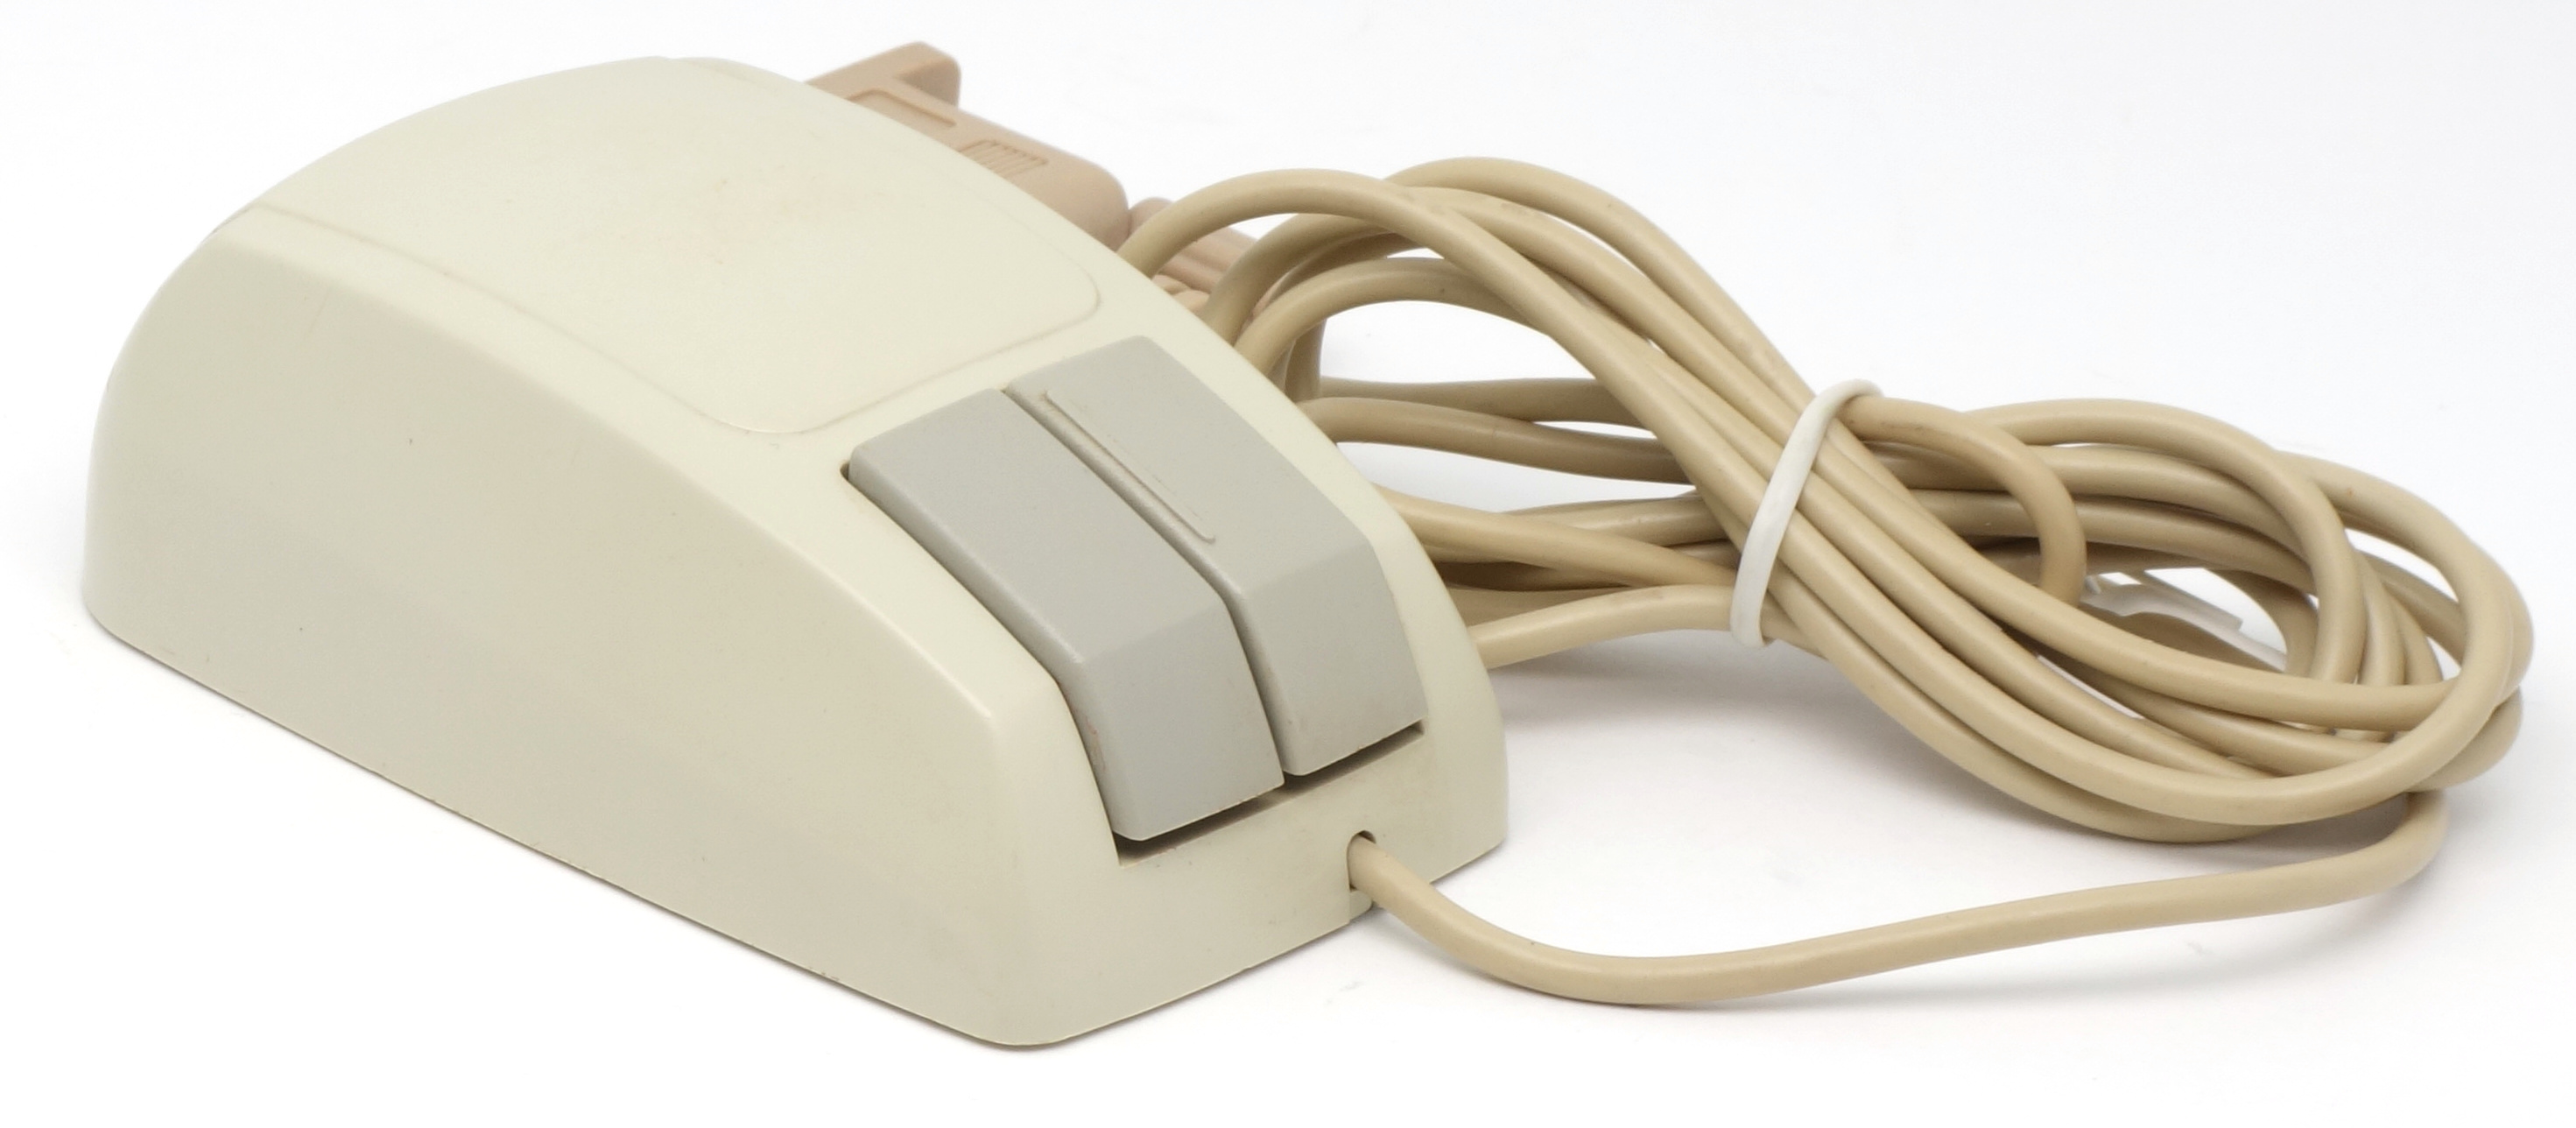
\includegraphics[scale=0.45]{1989_vatek_color_mouse/pic_30.jpg}
    \caption{Microsoft Gray-eyed Mouse}
    \label{fig:VatekColorPic}
\end{figure}

The device's body was made of red, green, yellow or blue plastic, but sometimes also of the standard beige \cite{mouses}, and was always equipped with two contrasting gray buttons. As you can see (fig. \ref{fig:VatekColorPic}), this particular ``color'' mouse is beige.

\begin{figure}[h]
    \centering
    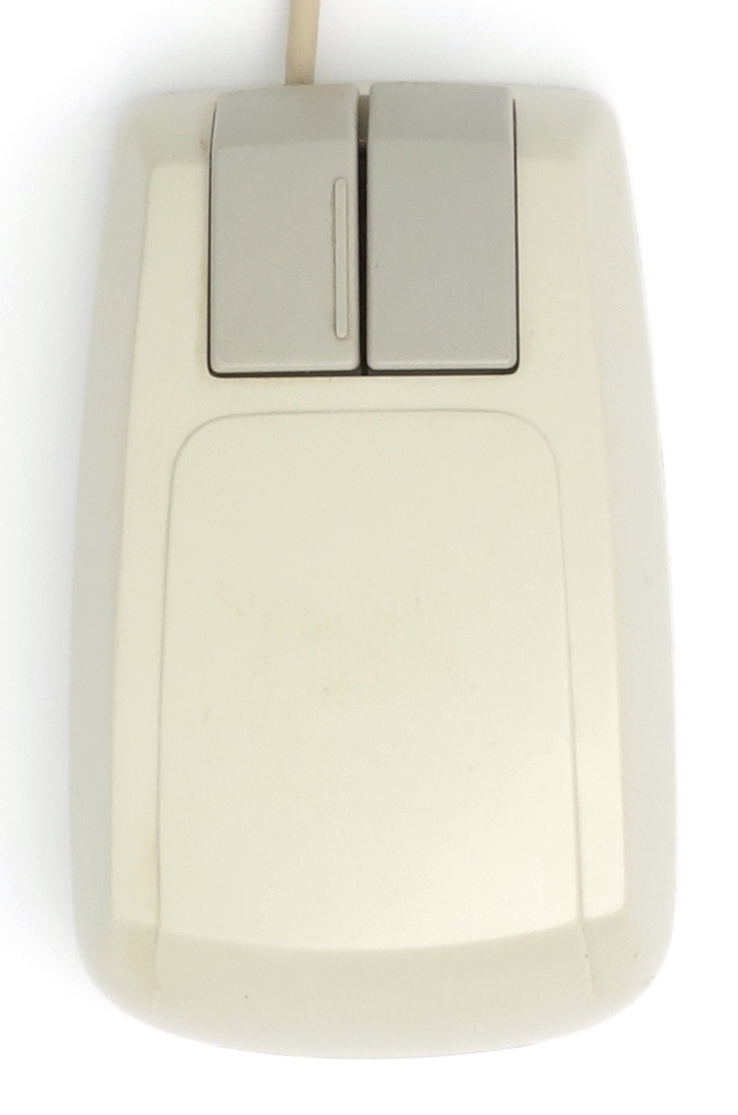
\includegraphics[scale=0.55]{1989_vatek_color_mouse/top_30.jpg}
    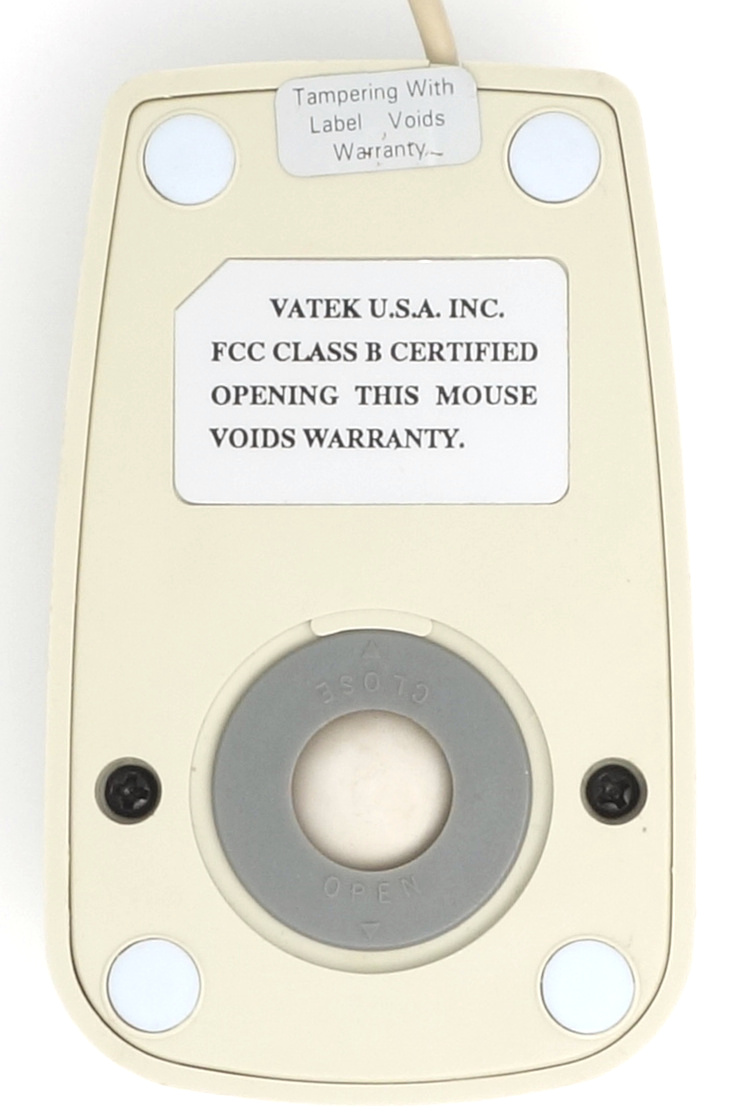
\includegraphics[scale=0.55]{1989_vatek_color_mouse/bottom_30.jpg}
    \caption{Microsoft Gray-eyed Mouse, top and bottom views}
    \label{fig:VatekColorTopAndBottom}
\end{figure}

The shape of the mouse copies the second generation Microsoft mouse released in 1985 (known as the ``gray-eyed'' mouse due to the color of the buttons). The top of the Vatek Color-Mouse body reproduces the body of the Microsoft mouse down to the point of identity, with the exception of wider buttons that are adjacent to each other (fig. \ref{fig:VatekColorTopAndBottom}). At the same time, the main button has a a small ridge on its right edge for easy tactile identification, which is borrowed from the third generation of Microsoft mice.
At the bottom, you can see a ball with a rubber coating, a locking ring that the user slides to remove the ball and clean the mouse, a plate with technical data (the FCC code is mentioned, but not shown), as well as four low-friction pads. The bottom side does not copy the ``gray-eyed'' Microsoft mouse (or rather, does not copy its typical ALPS design), except for the general silhouette and the position of the ball in the back of the body.

\begin{figure}[h]
    \centering
    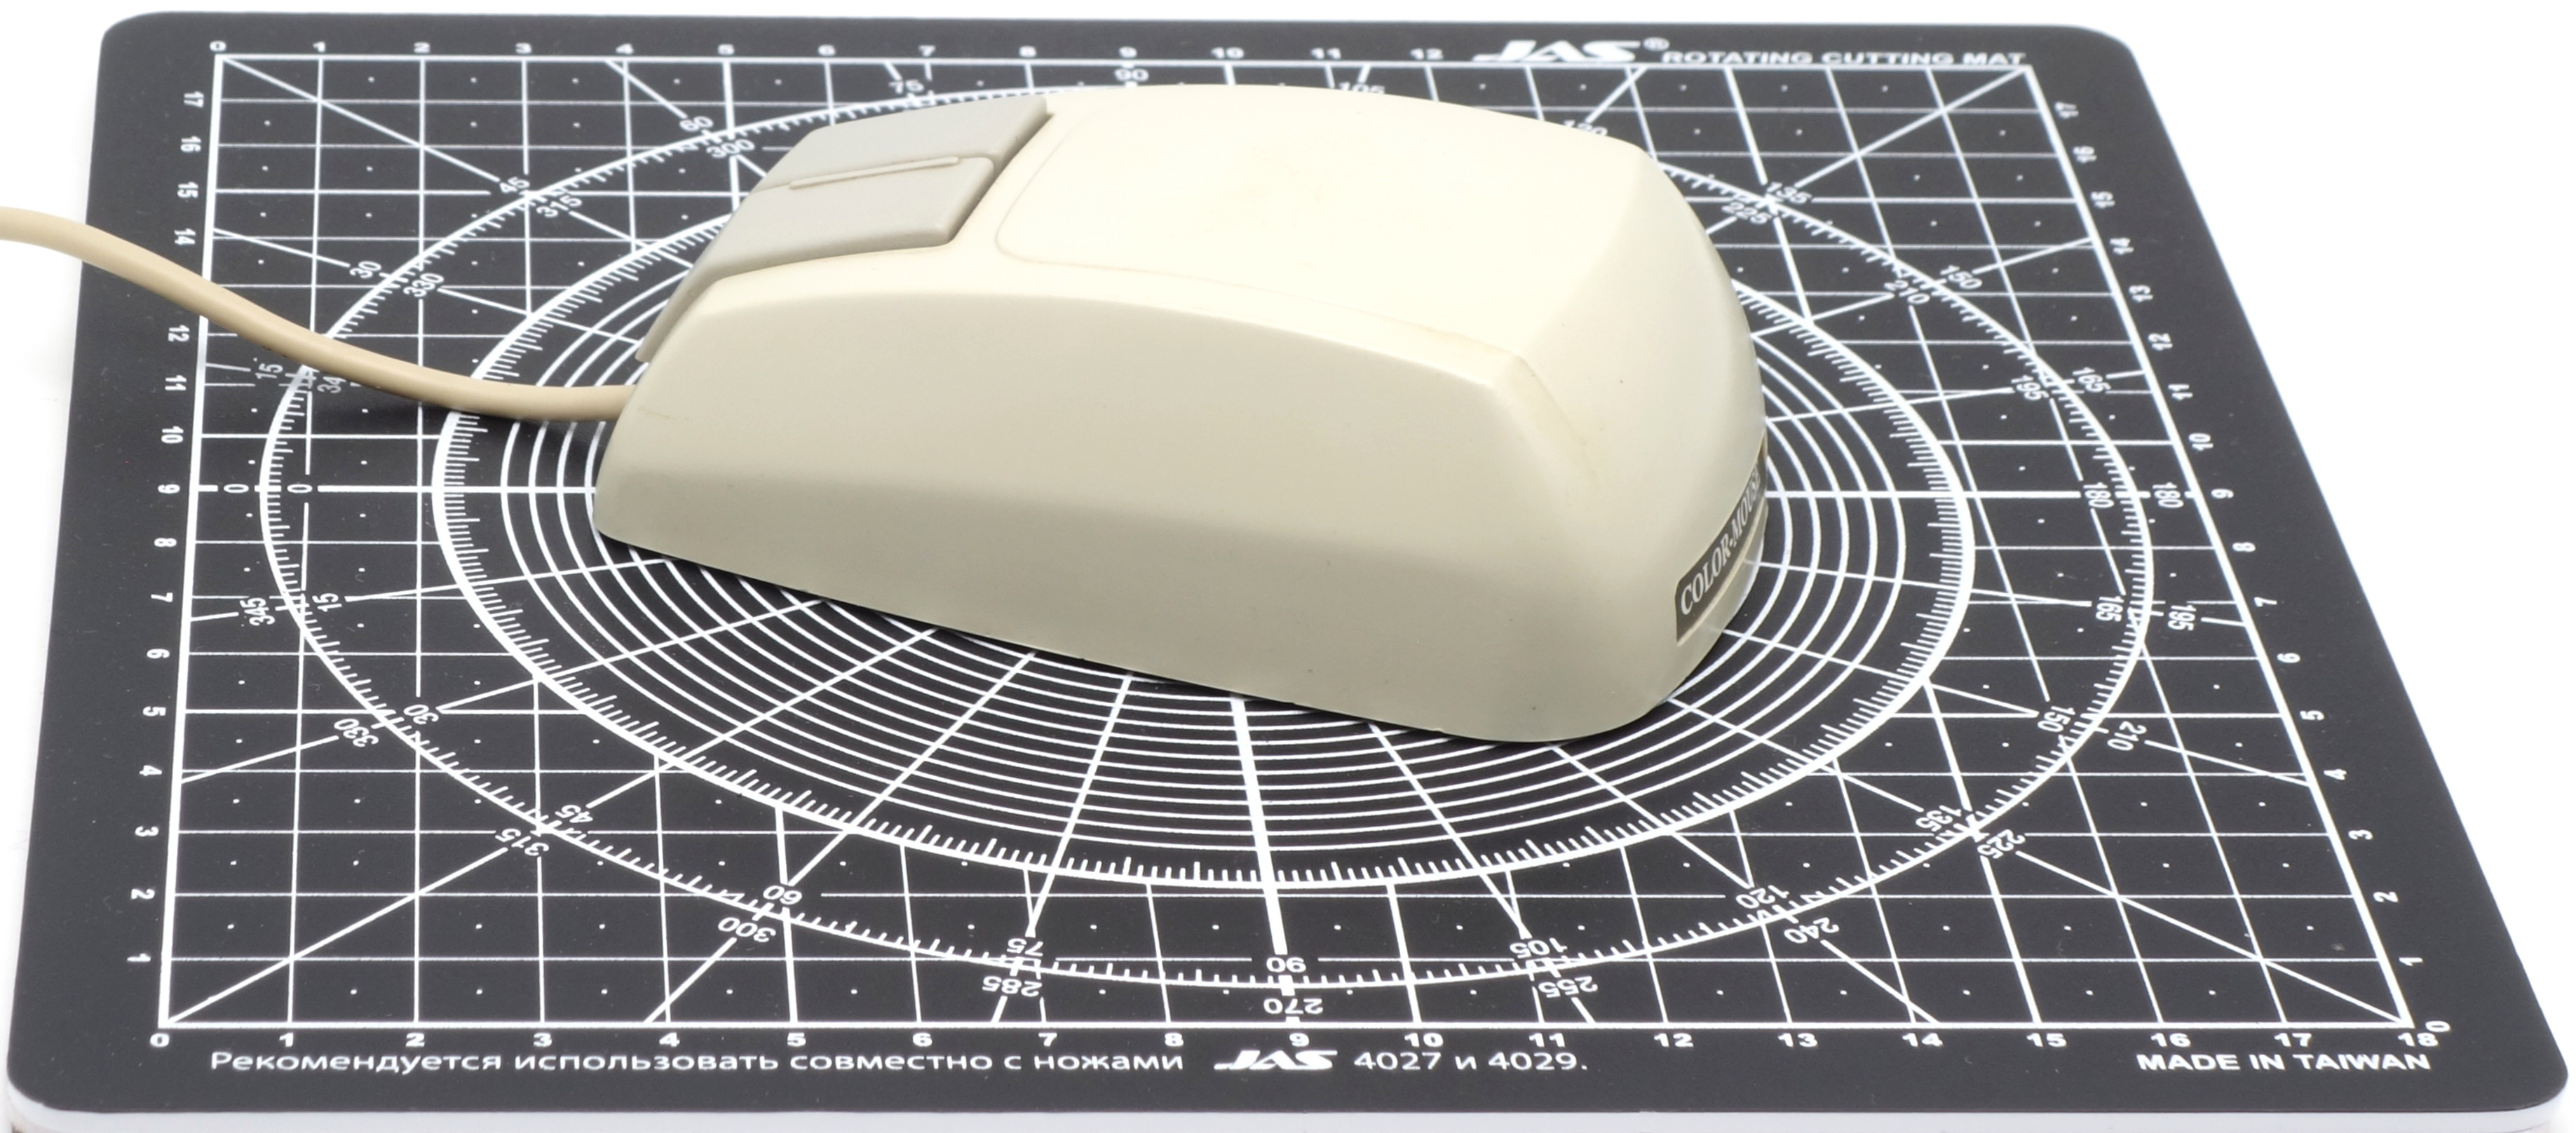
\includegraphics[scale=0.4]{1989_vatek_color_mouse/size_30.jpg}
    \caption{Microsoft Gray-eyed Mouse on a graduated pad with a grid step of 1~cm}
    \label{fig:VatekColorSize}
\end{figure}

For obvious reasons, the mouse dimensions were borrowed from Microsoft (fig. \ref{fig:VatekColorSize}), in whose case they were determined by the dimensions of the ALPS unit. In addition to the two-button Color-Mouse, a three-button mouse version was also released in the same case at the same time: it was sold under various brands, both well-known and unknown, and various names: Z-Nix Super Hi-Res Mouse, ProCorp Serial Mouse, SmarTEAM Smart Mouse, etc.

The ergonomics of the Color-Mouse also largely replicates the features of the Microsoft mouse, due to the same high body, convenient for gripping with a narrow palm, and angled buttons, slightly different for the better due to the fact that the Vatek buttons are wider. This angular shape of the buttons was invented by Microsoft as a logical development of the first generation mouse, the buttons of which were located on the body in front and caused criticism from some reviewers due to the possibility of accidentally moving the mouse simply by pressing them. In the advertising materials for the "gray-eyed" Microsoft mouse, it is mentioned that "the command buttons that wrap around the body are designed in such a way that they naturally fit in the palm of any size" \cite{mouses}, but obviously, such a double position of the buttons also solved the problem of erroneous movements, allowing those who find it more convenient to press them from above (Fig. \ref{fig:VatekColorHand}). Following Microsoft, this angular button shape appeared in some other mice, and the ones that are most similar to Microsoft, for obvious reasons, are the Vatek Color-Mouse and its three-button twin, known as the ProCorp Serial Mouse, etc.

\begin{figure}[h]
    \centering
    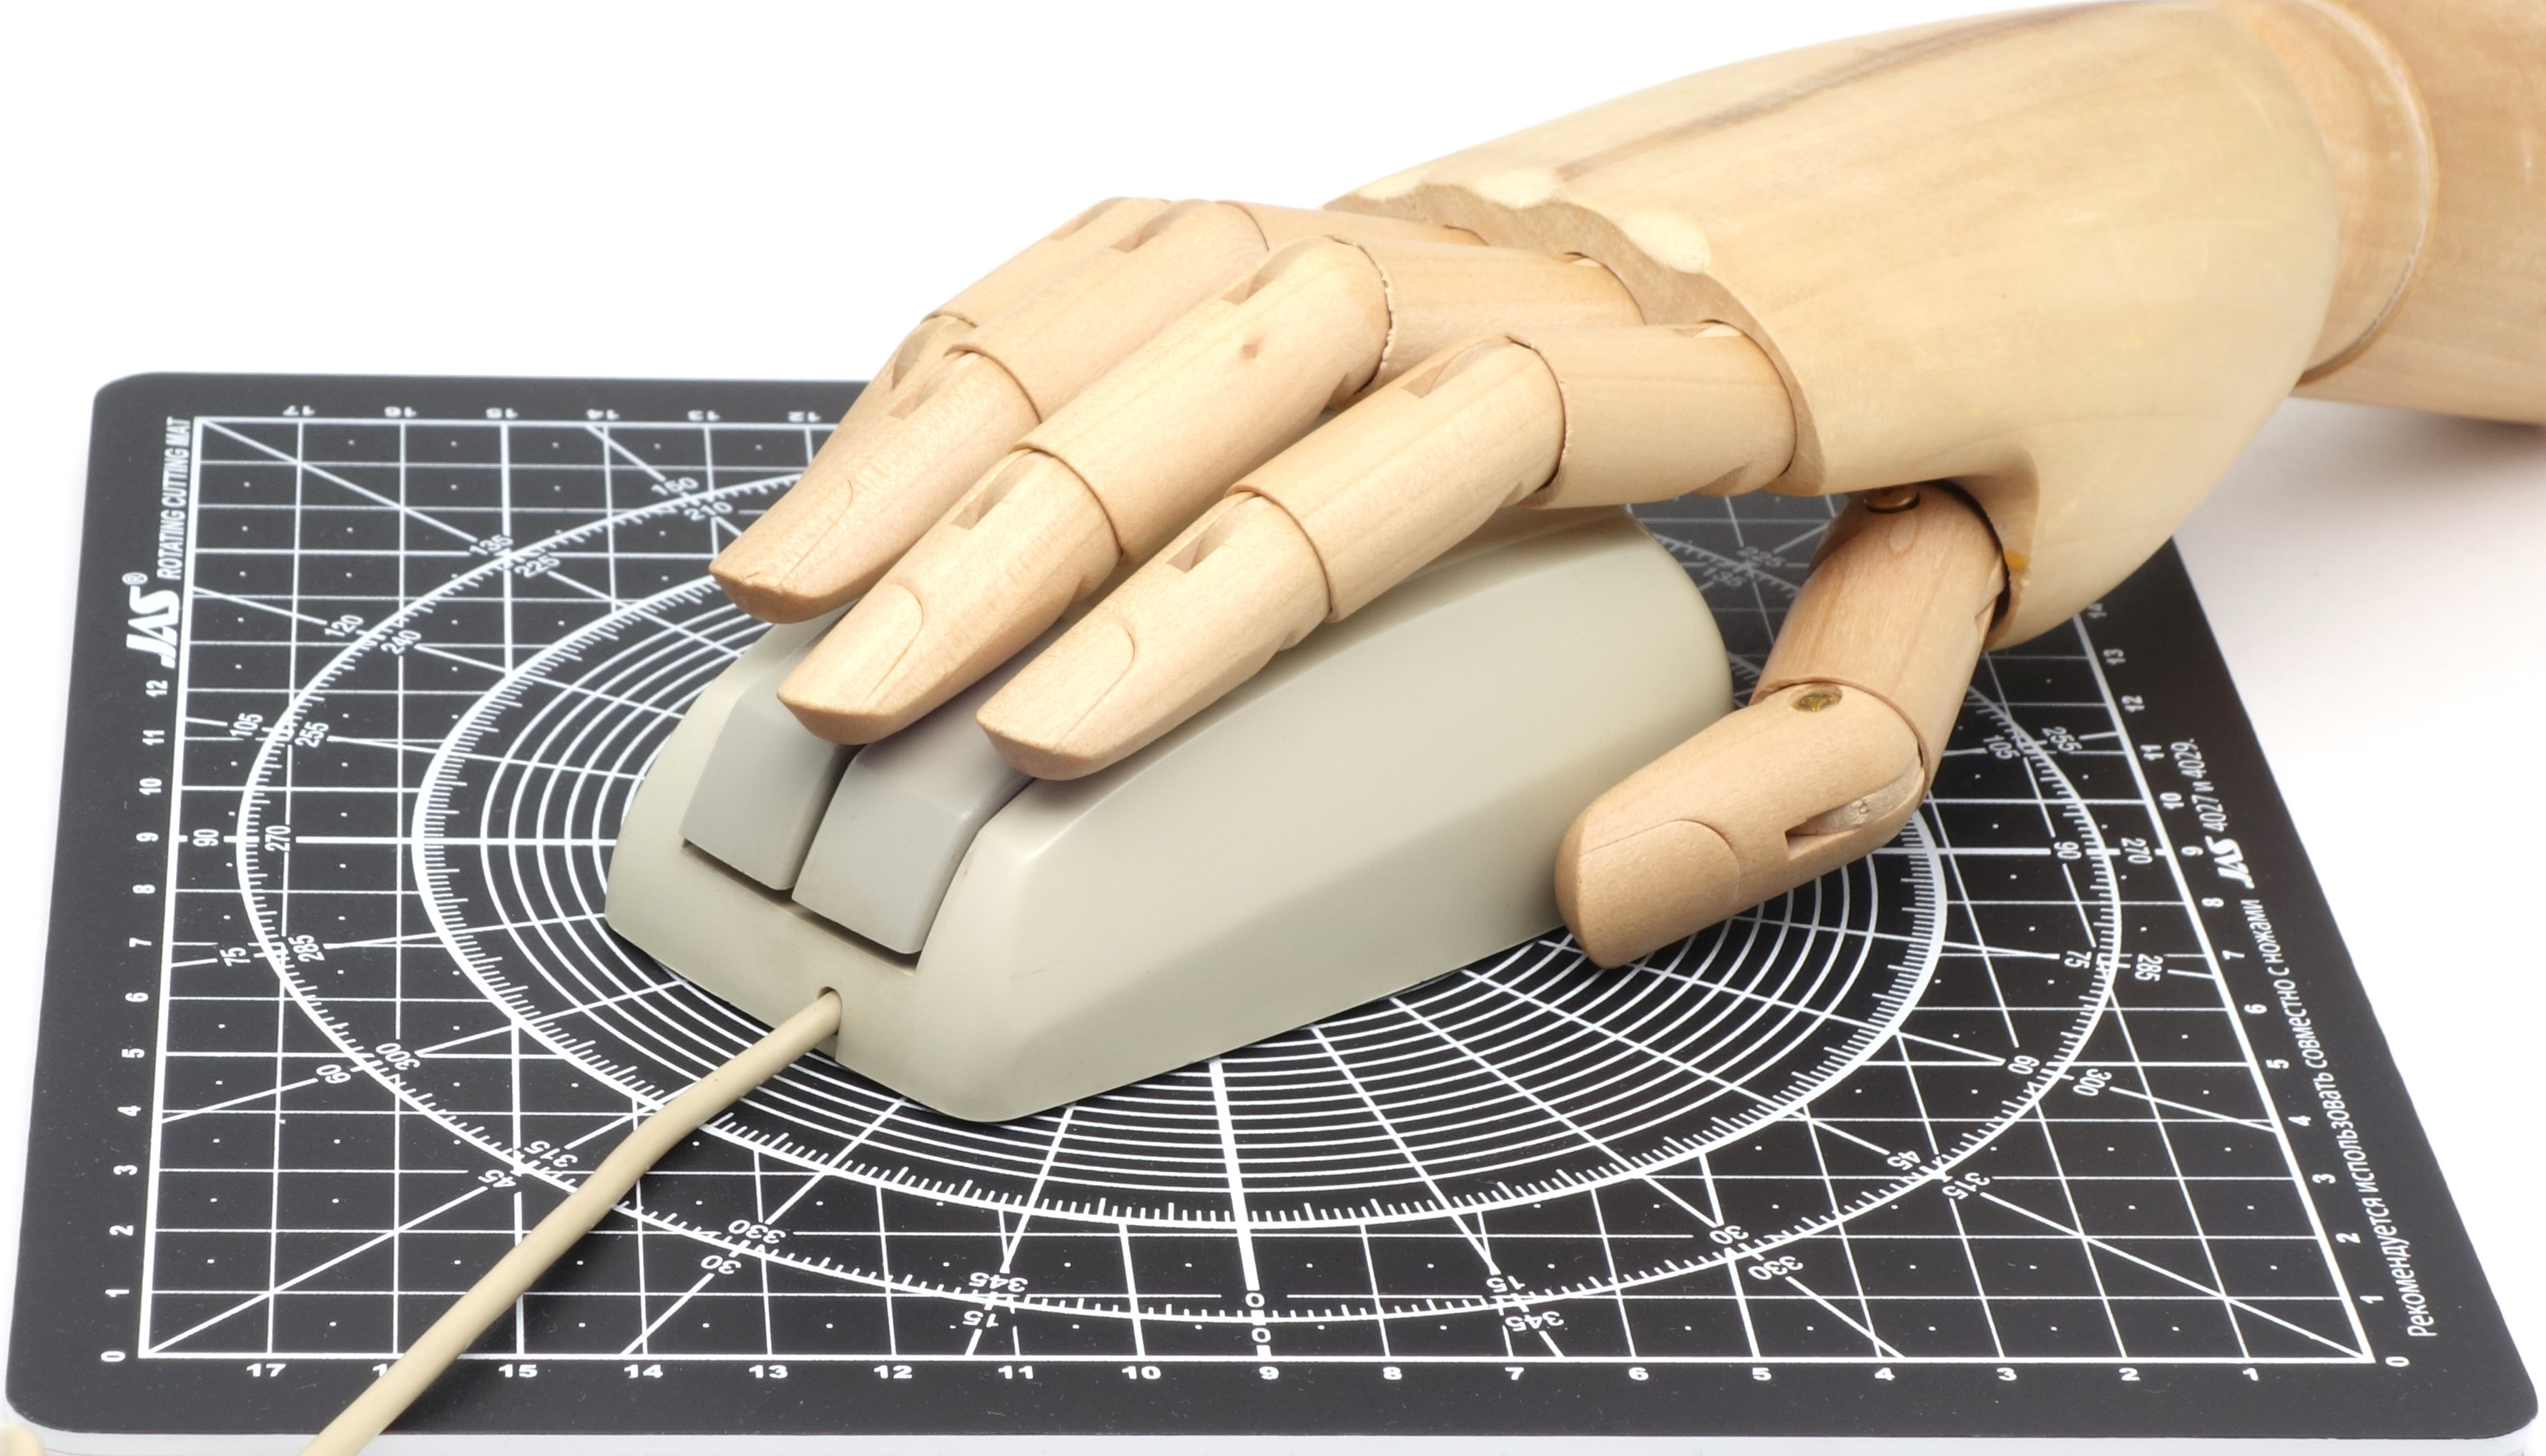
\includegraphics[scale=0.4]{1989_vatek_color_mouse/hand_30.jpg}
    \caption{Microsoft Gray-eyed Mouse with a human hand model}
    \label{fig:VatekColorHand}
\end{figure}

The Color-Mouse connects to a computer via a serial port using a 9-pin connector and has a rather modest resolution of 250 DPI\cite{dpi}.

An examination of the FCC ID code in the Federal Communications Commission database shows that the mouse was manufactured by Jow Dian Enterprise Co Ltd., a company registered in California. The FCC ID code was registered in 1988, but a similar code was also used for a three-button mouse. Earlier, Microsoft released two generations under one FCC ID code (the very first "green-eyed" mouse and the "gray-eyed" mouse, from which Jow Dian Enterprise borrowed the case shape). A comparison of the printed circuit board markings of the Color-Mouse and ProCorp Serial Mouse shows that the Vatek Color-Mouse was the second revision. Therefore, and according to \cite{mouses}, the mouse is dated 1989.

\begin{figure}[h]
    \centering
    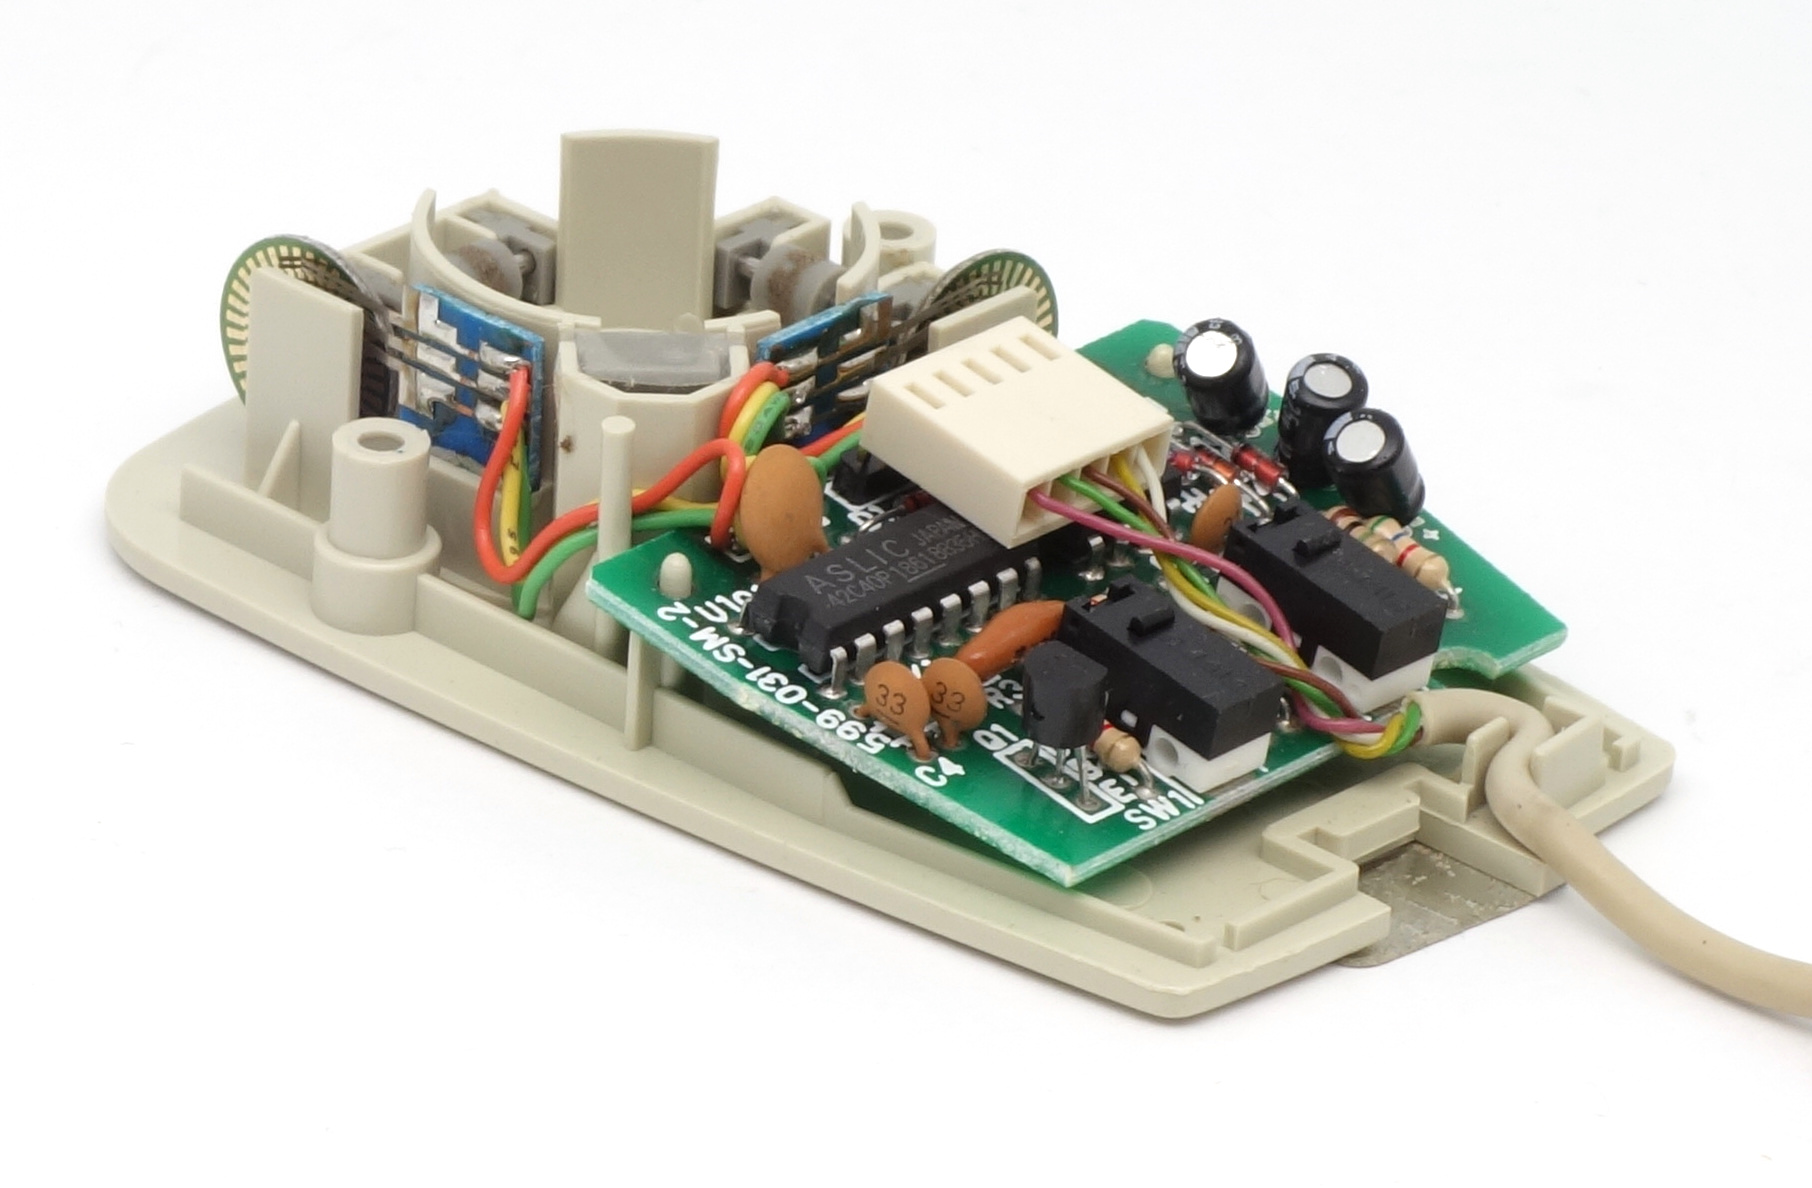
\includegraphics[scale=0.8]{1989_vatek_color_mouse/inside_60.jpg}
    \caption{Microsoft Gray-eyed Mouse disassembled}
    \label{fig:VatekColorInside}
\end{figure}

The internal structure of the mouse can be seen in fig. \ref{fig:VatekColorInside}. It is clear from the photo that the mouse has a mechanical encoder, like its prototype from Microsoft, but instead of the more reliable closed ALPS encoders, a budget option is used here - an open disk encoder, found in mice from the late 80s, more often intended for home computers of that time, simpler and cheaper than IBM PCs.

\begin{thebibliography}{9}
\bibitem{mouses} Vatek Color Mouse // Home Office Computing, December, 1989. -- P. 59 \url{https://archive.org/details/home-office-computing-december-1989/page/58/mode/2up}
\bibitem{company} Vatek USA * RMI Company Profile. \url{https://web.archive.org/web/19981201090808/http://www.vatek.com:80/company.html}
\bibitem{dpi} Color-Mouse // Dataquest: DQ, India: Cyber Media, 1990. p. 41.
\end{thebibliography}
\end{document}
